
\subsubsection{Classifier Performance}

We used a two-sample t-test to compare the AUC and MCR of the classifiers. The difference in classifier performance was statistically significant using both AUC and MCR as evaluation metrics (pauc = 7.2*10-10 and pmcr = 6.2*10-4). Both metrics indicated that $L_1$ regularized logistic regression is a stronger classifier for this task. Table \ref{table:liver_auc_mcr} shows the mean and standard deviations of the AUC and MCR.

For a more granular comparison of which semantic features were well-predicted, we looked at the AUC and MCR of each individual features. Figure \ref{fig:liver_auc} shows the area under the ROC curve (AUC) and figure \ref{fig:liver_mcr} shows the misclassification rate (MCR) of logistic regression with and without $L_1$ regularization.

\begin{table}[h!]
	\centering
	\begin{tabular}{|l|c|c|}
		\hline
		\multicolumn{3}{|c|}{\textbf{AUC statistics}} \\ \hline
		Classifier & Mean & Standard Deviation\\ 
		\hline
		LASSO & 0.816 & 0.141 \\ 
		\hline 
		Logistic & 0.584 & 0.098 \\ 
		\hline \hline
		\multicolumn{3}{|c|}{\textbf{MCR statistics} }\\ 
		\hline
		Classifier & Mean & Standard Deviation\\ 
		\hline
		LASSO & 0.1443 & 0.0881 \\ 
		\hline 
		Logistic & 0.2367 & 0.1085 \\ 
		\hline 
	\end{tabular}
	\caption{Aggregate statistics for classifier AUC}
	\label{table:liver_auc_mcr}
\end{table}


\begin{figure}
	\centering
	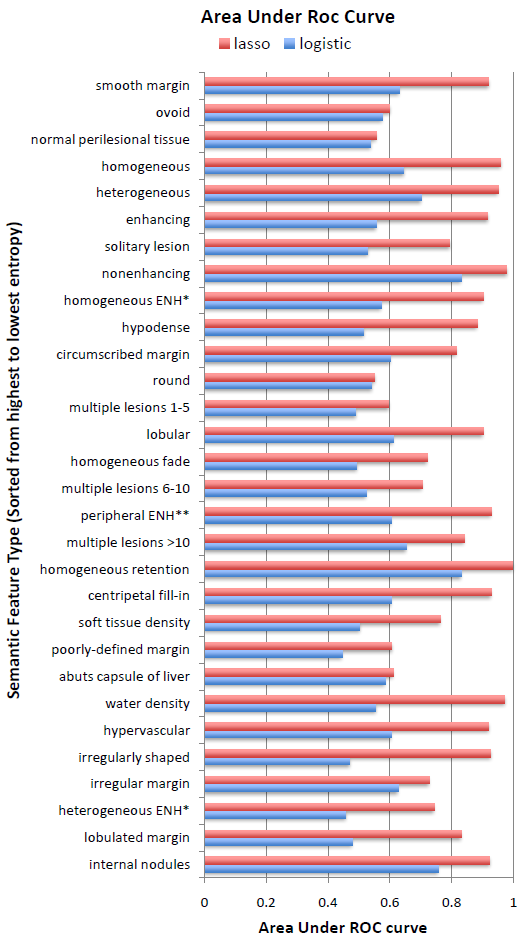
\includegraphics[width=\textwidth,height=\textheight,keepaspectratio]{liver_auc.png}
	\caption[AUC results for liver annotation]{Calculated area under the ROC curve given the probability of a semantic feature occuring for each lesion.Semantic features are ordered from highest to lowest entropy. ENH* = enhancement, ENH** = discontinuous nodular enhancement.}
	\label{fig:liver_auc}
\end{figure}


\begin{figure}
	\centering
	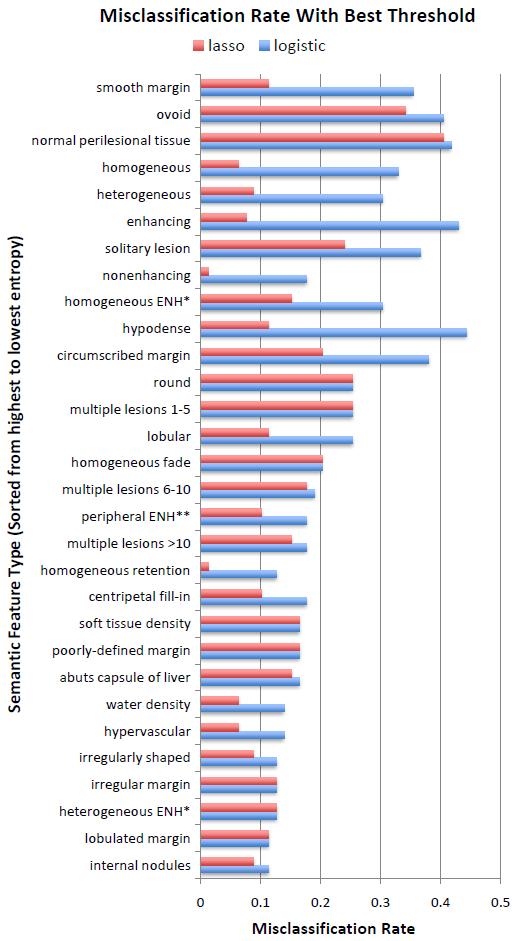
\includegraphics[width=\textwidth,height=\textheight,keepaspectratio]{liver_mcr.png}
	\caption[MCR results for liver annotation]{Misclassification rate using optimally determined threshold. Semantic features are ordered from highest to lowest entropy. ENH* = enhancement, ENH** = discontinuous nodular enhancement.}
	\label{fig:liver_mcr}
\end{figure}


\clearpage


\subsubsection{Semantic Features of Interest}
Using the LASSO classifier, several semantic features were shown to be well predicted given computation features. Five were found to have an AUC greater than 0.95: water density, homogeneous retention, non-enhancing, heterogenous, and homogenous.
Conversely, four semantic features were shown to have an AUC under 0.6: multiple lesions 1-5, round, normal perilesional tissue, and ovoid.

There were interesting results with regards to which semantic features were predictable. While we had developed several computational features to quantify shape, two of the most difficult semantic features to predict were round and ovoid. One possible reason for this discrepancy between computational and semantic features is that round and ovoid are inherently subjective terms. Hence, there might exist human variability in such descriptors that cannot be accounted for computationally. This explanation lends credence to further use of computational features for characterizing lesion shape, as there is no variability in our methods.

Another interesting result is our system's ability to predict seemingly impossible semantic features from one lesion. For example, ``multiple lesions > 10'' was very well-predicted even though analysis was carried out on only one lesion. Such results might be possible because there is an explanatory disease behind both lesion morphology and multiple lesions. Thus, we can indirectly predict number of lesions based on analysis of a single lesion's physical characteristics alone.

\subsubsection{Computational Feature Analysis}
Computational features were fitted to each semantic feature vector using the LASSO model. Each fit produced a 431-dimensional set of weights for the computational features. Features with large magnitude weights were deemed most informative.  The L1 norm regularization in the model imposes a sparse weight selection; most features have zero weight. To quantify the model complexities, we fit a lasso model to each semantic feature group and counted the number of non-zero coefficients. This corresponds to the number of relevant computational features in each semantic feature group. On average, each semantic feature only employed 12.6 ($\pm$ 4.3) computational features. Moreover, of the entire set of 431 computational features, only 126 computational features had non-zero for any semantic feature vector.

Computational features that consistently had high magnitude weights were considered as characteristic features of these lesions. Characteristic features were found by taking the sum of the absolute value of weights across all semantic features. The 20 features with highest sum of weight magnitudes were categorized according to their associated algorithms. Daubechies Wavelets, Edge Sharpness, Gabor Transform, and the Local Area Invariant Descriptor were found to be the most informative feature groups.
